
\documentclass[10pt,twocolumn,a4paper]{article}
\usepackage{styles/usenix-style}

\author{Fabian Nguyen}


\usepackage{cite,xspace,ifthen,graphicx,listings}
\usepackage[font=small,labelfont=bf]{caption}
\usepackage[
   pdfauthor={Fabian Nguyen},
   pdftitle={Advanced Exploit Mitigation},
   pdfsubject={Windows Internals},
   pdfkeywords={Security,Stack Overflow,Return Oriented Programming, Control Flow Guard, Shadow Stack}
]{hyperref}
\usepackage[nonumberlist, section]{glossaries}
\usepackage{hyperref}

\begin{document}

\title{Windows Internals: Advanced Exploit Mitigation}

\newcommand{\todo}[1]{{\texttt{[#1]}}}
\newcommand{\code}[1]{{\tt \small{#1}}}

\maketitle


\begin{abstract}
We take a look at general techniques used by attackers to compromise Windows systems and some fundamental defense mechanisms against them.
This paper will provide an overview of Microsoft's latest additions to the security concept of the Windows Operating System [OS] , analyse inherent flaws in their design and take a brief look at already existing attacks. 
\end{abstract}

\section{Introduction}\label{sec:introduction}
In an increasingly digitalized world an overwhelming amount of private and/or safety-critical information and data is stored on computers.
Windows is by far the most used operating system and therefore the main target of attackers to compromise data or computer systems.
One common intent of attackers is to steal an individual's passcode e.g., for an online-banking website.
Naturally, as the amount and complexity of attacks rises, OS vendors are forced to put an increasingly high amount of effort into mitigating existing weaknesses and deny attackers of further possibilities to compromise their OS.
Even though this is the case, the amount of potentially abusable vulnerabilities in Windows has been increasing, instead of decreasing.

\begin{figure}[h]
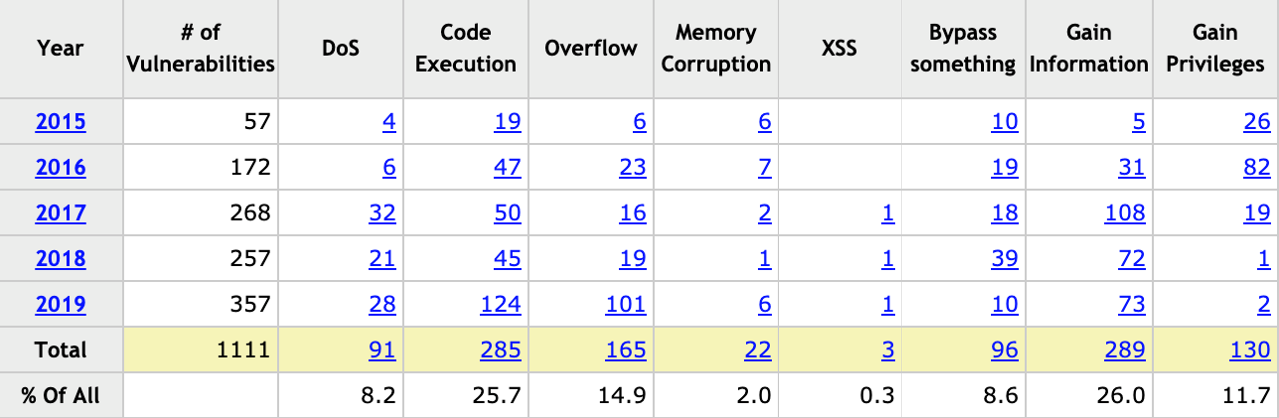
\includegraphics[width=8cm, height=2.5cm]{fig/stats}
\caption{Amount of documented vulnerabilities in the Windows Operating System.\newline Note that the spike in "Gain Information" vulnerabilities in 2017 is inflated by a family of attacks widely known as Meltdown/Spectre \cite{CVE}}
\end{figure}

We can see that the three largest groups of vulnerabilities consist of "Gain Information", "Code Execution" and "Overflow".
Of course these three categories aren't entirely separated from each other.
An attacker that is able to execute code on a machine often does so in order to gain information and overflows are often the reason why an attacker can execute code in the first place.
We'll take a quick look at how these issues play together and what has been done against them in the past before taking a deeper dive into Microsofts newest defense additions.

\section{Overflows}\label{sec:Overflows}
An overflow happens when a program writes data to memory beyond the limits of the intended data structure.
One common example of this is a stack buffer overflow caused by an incorrect use of the function \emph{strcpy}.\footnote{"char * strcpy ( char * destination, const char * source )" is a C function that copies a string into the specified memory}
More precisely, an overflow can occur when the given input is longer than the buffer one writes to.
\begin{figure}[htbp]
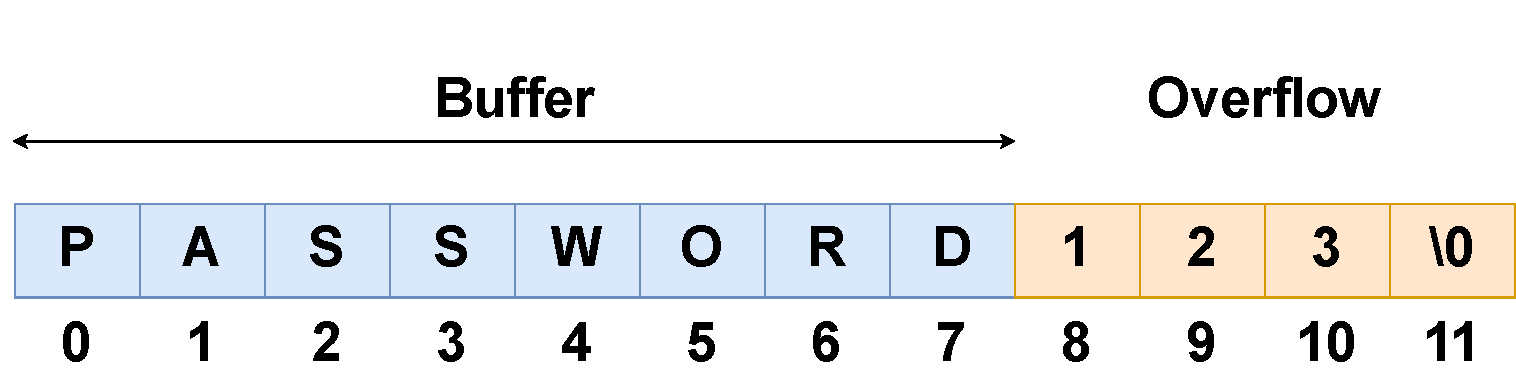
\includegraphics[width=8cm]{fig/simpleoverflow}
\caption{The password's length is too large to fit into the designated buffer.However, strcpy will not check for valid sizes so it will continuously write beyond the buffer.}
\end{figure}
\newline Relatively small-in-size overflows are not always easy to spot and often remain unidentified if they don't cause immediate errors.
In addition to causing faulty program behaviour, this also provides a critical attack surface.
To see why this is the case let's take a look at a typical stack layout with only one buffer present right at the beginning.
\begin{figure}[h]
	\begin{center}
		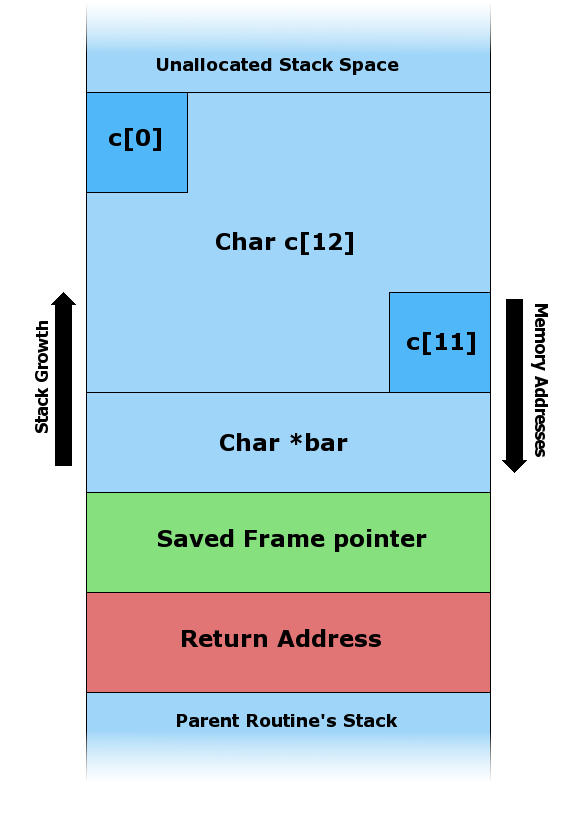
\includegraphics[height=7cm,width=6cm]{fig/Stack_Overflow}
		\caption{A typical stack layout}
	\end{center}
\end{figure}
\newline
As we can see the stack will usually contain a return address right at the bottom, a frame pointer on top of it, and then local data that is used by the current function.
Obviously one will also need to keep the parent function's data saved below (stack grows upwards).
In our example there is only one character buffer of size 12 and a pointer to it present.
Suppose one wants to copy user-input string into this buffer e.g., by using \emph{strcpy}.
The user may now unknowingly or perhaps purposely overflow this buffer by entering a string that's longer than 12 characters.
As we observed earlier this will result in a memory-write beyond the buffer's bounds. 
\begin{figure}[h]
	\begin{center}
		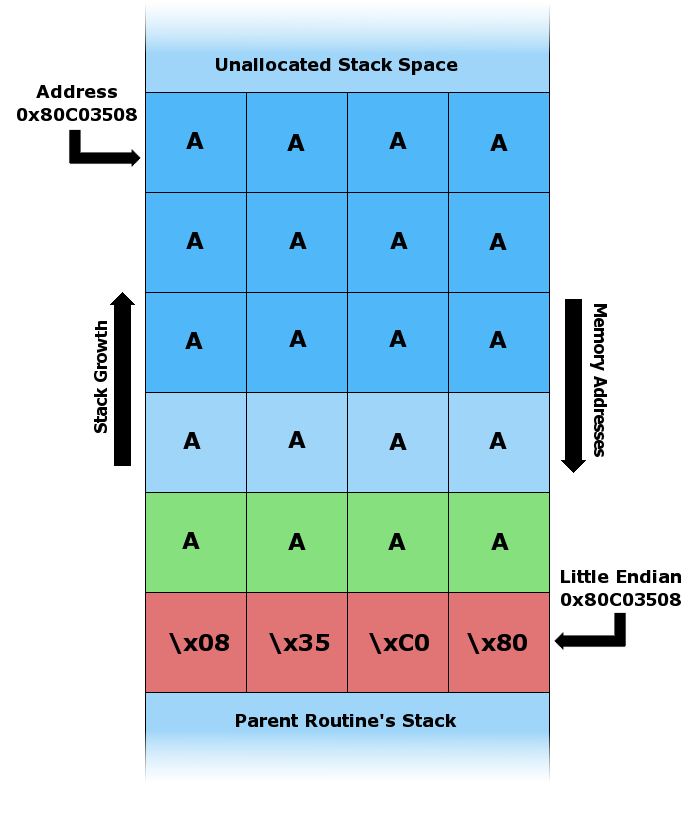
\includegraphics[height=7cm,width=8cm]{fig/Stack_Overflow2}
		\caption{The user-input is too long for the given buffer}
	\end{center}
	\end{figure}
\newline 
In this example, we can see that our pointer to the buffer is overwritten, as well as the stack frame we had saved on the stack earlier.
Most importantly though, the return address is also corrupted.
In the given figure, the input is constructed so that the part that's written over the return address resembles an address itself.
In this case, it's just the address of the buffer again.
At some point, our given function will attempt to return to this address.
However, once it does so, all it will be able to read from this address is a swarm of  'A's which certainly doesn't resemble a valid sequence of code.
The program will fault and terminate.
This problem has existed for as long as the concept of the stack itself so naturally techniques to (try) prevent this from happening were implemented long ago.

\section{Data Execution Prevention}\label{sec:DEP}
One easy and naive way to address the aforementioned issue is the use of Data Execution Prevention (DEP).
DEP follows a very simple approach to prevent the execution of code from malicious addresses.
Note that an attacker that uses overflows can usually only manipulate the stack which is typically used for non-executable data only.
Since we know that, we could easily mark the entire memory-area\footnote{Sometimes code needs to be run directly from the stack e.g., just-in-time compiled JavaScript code, so this is a very simplified approach} (with an additional attribute for memory pages) that is used as a stack as \emph{non-executable} or "NX" in short and that is basically what DEP does.
Whenever an attempt to run code is made a check will ensure that the "NX"-Bit for the according page is not set.If it is, the program will terminate immediately.
This approach offers an easy solution to prevent the \emph{execution} of code on the stack.
However, it does \emph{not} prevent an attacker from redirecting control flow to already existing code. Attacks that abuse this flaw could therefore still compromise or even take over a program.\footnote{A well known way to do this is a \hyperref{https://en.wikipedia.org/wiki/Return-to-libc_attack}{Return-to-Libc Exploits}{name}{return-to-libc attack}}

\section{Address Space Layout Randomization}\label{sec:ASLR}
Address Space Layout Randomization (ASLR) was implemented to address this issue.
Since an attacker that uses pre-existing code needs to be able to tell where the code they want to use is, an easy solution is to prevent them from addressing said code.
ASLR does this by randomizing the arrangement of segments like the stack, heap and DLLs in memory. This means that using a fixed address to reference memory will most likely result in a segmentation error or the wrong code being targeted at best.\footnote{32 bit Windows randomizes 8 of the address' bits, 64 Bit Windows can randomize a total of 19 bits.} However, a single pointer leak may compromise the location of any of the segments and thus break ASLR completely. (Note that this has happened quite often already)

\section{Return Oriented Programming}\label{ROP}
Return oriented programming describes one of the most popular approaches to manipulating programs by hijacking control-flow through the manipulation of return addresses.
In essence, there are three steps to do :
\begin{enumerate}
	\item Finding a security vulnerability that allows one to manipulate memory
	\item Writing code (also called Payload or Shellcode\footnote{The name Shellcode comes from the fact that such attacks often inject code to open a Shell on the target system} on the stack 
	\item Manipulating the return address to point to the injected code
\end{enumerate}
Windows did not offer any kind of protection against ROP attacks until 2004 when DEP was introduced.
However, as already mentioned, attackers quickly overcame this barrier by using already existent code which would not be marked non-executable.
One proposed "solution" to this was to store the first argument of each function in a register instead. Registers are not as easy to manipulate due to not being explicitly writeable in theory, though attackers easily overcame this restriction as well.
Instead of using complete functions they would now use only small portions of a function that ended in a return instruction. Obviously, instruction sequences that allowed to manipulate registers were especially useful, in order to invoke complete functions again.
However, this is not needed as the usage of such so called "gadgets" is already turing-complete given a \emph{big enough}\cite{gadgets} program.
This is made even easier by the fact that one can use instruction sequences that weren't supposed to be in the program to begin with.
To see how this is possible, recall how machine code is written and read by the CPU.
Note that in contrast to natural language, machine code doesn't include any white space (e.g., spaces or slashes) so one may start reading wherever they want.
The following figure shows an example where two instructions are split into four just by removing one byte at the start.
\begin{figure}[h]
  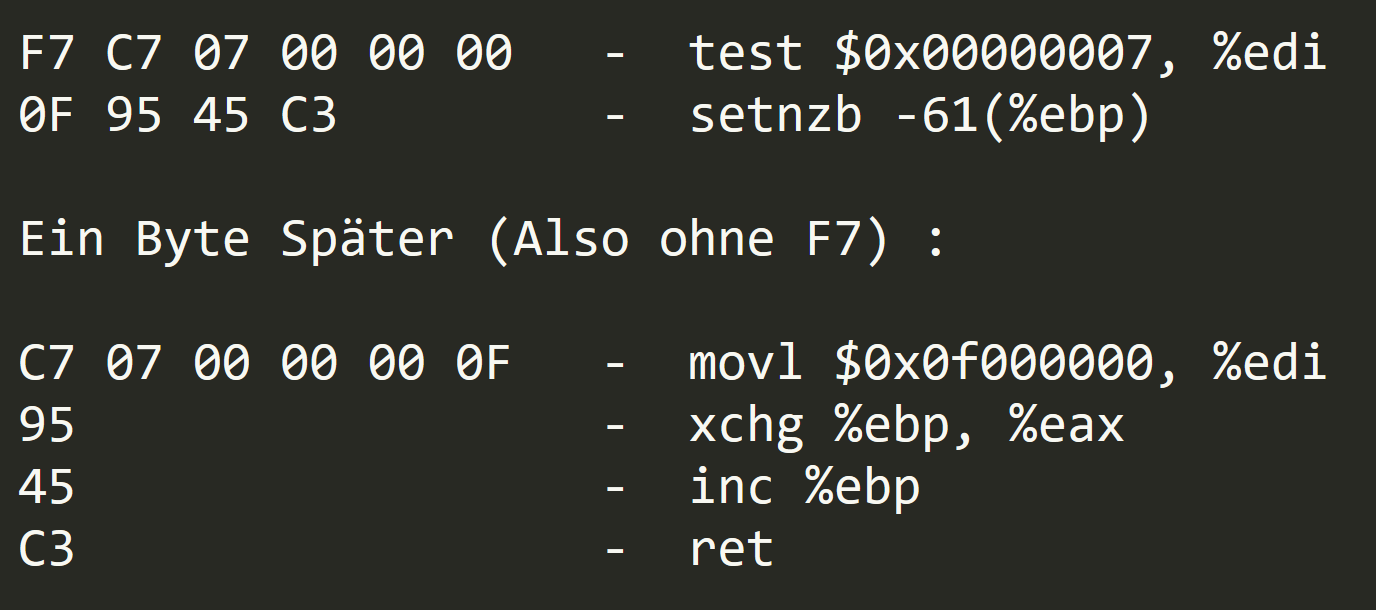
\includegraphics[keepaspectratio,width=8cm]{fig/ByteCode}
  \caption{An example of an unintended use of machine code \cite{geometry}}
\end{figure}
\newline
In theory, ASLR should prevent such attacks completely since no attacker should be able to locate any specific code to begin with.
In reality though, vulnerabilities in both DEP and ASLR (even combined) have been found and successfully exploited.
How this was done won't be covered here, but it's important to see that these techniques weren't sufficient protection after all.

\section{Shadow Stack}\label{shadowstack}
The idea of a Shadow Stack follows a different approach to the issue.
Instead of trying to prevent the manipulation of the return address an additional check is built in to make sure it wasn't altered.
In order to do this, the Shadow Stack saves all return addresses in a separate memory location.
Every call instruction in a program pushes the return address of the parent routine on the normal stack \emph{and} on the Shadow Stack.
Every return instruction pops one address off the Shadow Stack and compares it to the address on the normal stack.
Note that calls to exception handlers and \emph{longjmp}s may cause issues here as calls and returns aren't necessarily perfectly matched if they occur\cite{light}.
One solution to this is to continuously pop addresses off the shadow stack until a matching address is found. In this case, a program would be terminated if the shadow stack runs empty without match.
Implementing special treatment for these troublesome calls instead would increase runtime performance but include a higher memory overhead and increase complexity.
\begin{figure}[h]
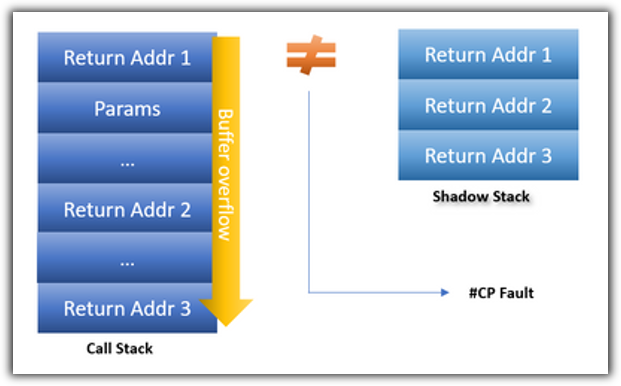
\includegraphics[keepaspectratio,width=8cm]{fig/Shadow Stack}
\caption{Shadow Stack Overview}
\end{figure}
\newline
In order to do this, a new register called Shadow Stack Pointer(SSP) and an additional memory page attribute are used.
Writes to the Shadow Stack are restricted to control transfer instructions(\emph{call/ret)} and Shadow Stack management instructions for obvious reasons.\footnote{There's no point in having a separate stack to save data when its explicitly writeable}
Note that this approach only provides integrity of "backward jumps" (also called Backward Edge)."Forward jumps" may still be manipulated while a Shadow Stack is being used. We will come back to this in a bit.
\subsection{Shadow Stack revisited}
One main problem with the Shadow Stack is that virtually no one is able to make use of it as of now. Since Microsoft's implementation of the Shadow Stack requires an additional register it is only usable with certain CPUs (more specifically those using a chipset that supports Intel Control-Flow-Enforcement technology).
Intel's first generation of CPUs that use this chipset are yet to be released\footnote{Intel Tiger Lake CPUs are announced for late 2020} and so are AMD's.
\newline ARM won't be releasing any compatible CPUs\cite{techrepublic}.
Additionally, once compatible CPUs are released it will still take a couple of years for them to be used widely.
Considering that a software version of the Shadow Stack (dubbed Return Flow Guard) was already in development it is not quite apparent why this approach was not further pursued.
According to unofficial sources \footnote{https://www.techrepublic.com/article/windows-10-security-how-the-shadow-stack-will-help-to-keep-the-hackers-at-bay} development of the RFG was discontinued because a vulnerability in the implementation was found. Surely something could've been done about this in the meantime though. An imperfect mitigation is better than no protection after all.
One good aspect is that optimized Shadow Stacks have a runtime overhead of at most five percent and negligible memory overhead.
Note that the Shadow Stack only validates return addresses though. Function parameters are (intentionally) not protected. This is essentially a trade-off between security and runtime/memory overhead. It is non-trivial when or whether this trade-off is worth it and surely depends on the intended environment.
Lastly, according to Microsoft the use of Shadow Stacks will be opt-in "at first" per linker-flag for apps and DLLs for compatibility reasons.This will further increase the time needed for CFG to spread.

\section{Control Flow Guard}\label{CFG}
To take care of the Forward Edge the Control Flow Guard was shipped with Windows 8.1 Update 3.
More specifically, CFG aims to prevent the misuse of indirect jumps.
To do this developers can compile their programs with the CFG flag and ensure that their program will only run on memory areas that have been marked "safe" earlier.
Here, "safe" means that the address of every indirect jump refers to a valid function in the program.
In order to check this efficiently at run time, a bitmap of the starting addresses of every function is created at compile time where every bit in the bitmap corresponds to 8/16 \footnote{8 bytes per bit at first, later changed to tuple per 16 bytes} bytes in the address space.
If a function starts within the block of addresses that correspond to a given bit it is set to '1', otherwise it is '0'.
A guard instruction is then inserted before every indirect jump which validates that the matching bit for the target address in the bitmap is set to 1. If it is not, the program is terminated immediately.
\begin{figure}[htbp]
	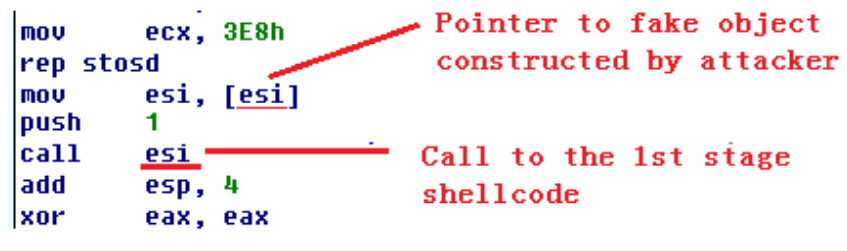
\includegraphics[keepaspectratio,width=8cm]{fig/nocfg}
	\caption{Example code without CFG\cite{cfgexplore}}
	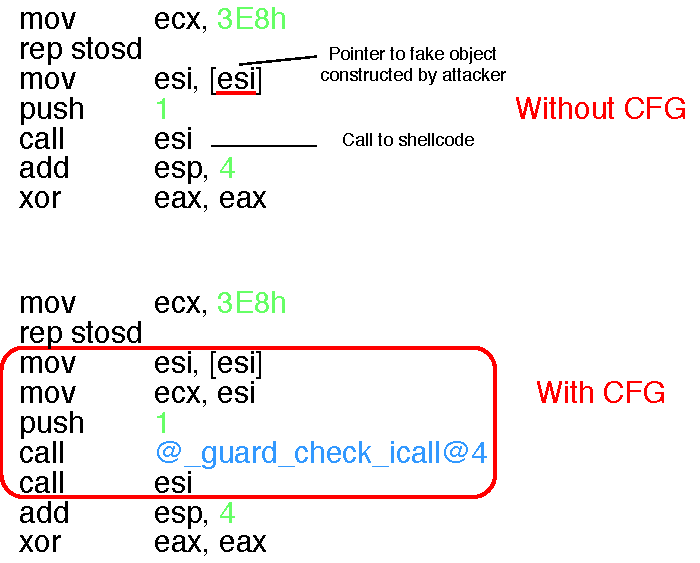
\includegraphics[keepaspectratio,width=8cm]{fig/cfg}
	\caption{Example code with CFG enabled}\cite{cfgexplore}
\end{figure}
If a CFG compatible program is run on a Windows version that doesn't support CFG the call simply does nothing.
To increase performance, system processes which are run as "protected" processes use shared bitmaps for DLLs.
Note that dynamically generated functions cannot be protected this way as explicitly allocated and \emph{executable} marked memory has its corresponding bits in the bitmap implicitly set to 1.
This is because dynamically allocated memory can not be considered at compile time.
\subsection{Control Flow Guard revisited}
One major flaw in the initial design of CFG lies in one of its main assumptions: That the addresses of functions are aligned to eight bytes.
While this assumption holds true for the compiled program itself (since the compiler can enforce the alignment) it certainly is not for DLLs.
To make up for this issue the CFG uses a mapping of two bits (a tuple) for every 16 bytes since Windows 10 instead where (0,0) means no function starts in the corresponding address block, (1,0) means a function starts at the start of the block and (1,1) means a function starts anywhere in the block.
Note that this still provides a sort of margin for attacks when alignment is not enforced as an attacker can still manipulate a jump to point to anywhere within a (1,1) block (15 bytes of unintended viable targets in the worst case!).
\begin{figure}[h]
	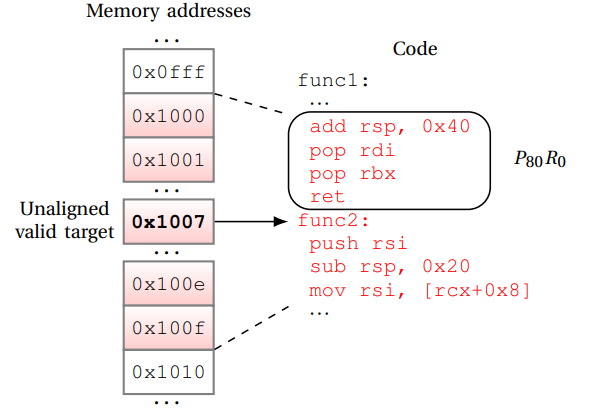
\includegraphics[keepaspectratio,width=8cm]{fig/cfgunallignedcode}
	\caption{An example of why unaligned addresses can be a major vulnerability\cite{cfgexplore}}
\end{figure}\newline
Another oversight that was found rather quickly: The guard function wasn't properly protected.
In 2015 Zhang Yunhai showed that by using a (custom-)heap-allocation and freeing it afterwards one may make its memory area writeable again under certain circumstances.\cite{cfgbypass}
Last but not least another major issue that has not been fixed as of now:
Lots of Windows system DLLs are not compiled to use CFG (145 in Windows 10 1511 / still 50+ in build 18362).\cite{cfgbypass2}
Note that any program, even if it is compiled to use CFG, is vulnerable when it uses a DLL that is not, since the guard calls are only present for the CFG compiled program.
This means that as long as there are unprotected modules present every part of the program is vulnerable.

 %\begin{figure}[htbp]
%  \centering
%  \fbox{\parbox{.8\columnwidth}{
%      Here you can include a sample figure.  Use something like
%      \begin{center}
%        \code{$\backslash$includegraphics[scale=.8]\{template\}}
%      \end{center}
%      to include an encapsulated postscript figure.  The \emph{scale}
%      argument can be used for scaling the picture, although it
%      may scale the font incorrectly.
%    }}
%  \caption{Sample Figure}
%  \label{fig:sample}
%\end{figure}


%\lstset{language=C, basicstyle=\ttfamily,
%        string=[b]', showspaces=false, showtabs=false,
%        caption={A sample code snippet}, captionpos=b}
%\begin{lstlisting}
%/* code snippet  */
%while (!sleep)
%	sleep++;
%\end{lstlisting}

%\begin{figure}[hbt]
%\centering
%\includegraphics[scale=.7,clip]{fig/OIUKAvV}
%\caption{Sample figure automatically from Windows prn.\label{plot:fig}}
%\end{figure}
 

\section{Approach}

\section{Conclusion}\label{sec:conclusion}



\bibliographystyle{ieeetr}
\bibliography{AdvancedExploitMitigation}
%\size
\end{document}